\documentclass{article}
\usepackage[utf8]{inputenc}
\usepackage{amsmath}
\usepackage{listings}
\usepackage{graphicx}

\graphicspath{{/home/pdro/Prog/introFISCOMP/2}}

\title{Projeto 2: Decaimento radioativo e números aleatórios}
\author{Pedro de Carvalho Braga Ilídio Silva - 9762595}
\date{Abril de 2017}

\begin{document}

\maketitle

\section{Introdução}

O presente projeto visa o estudo da implementação de números pseudo-aleatórios na linguagem de programação Fortran90. Serão criados e analisados geradores congruentes lineares. Em um segundo momento, será estudada uma aplicação típica: o processo de decaimento radioativo para uma determinada quantidade de amostras de núcleos instáveis. Gráficos do decaimento serão elaborados e sua natureza, discutida.

\section{Desenvolvimento}

\subsection{Números aleatórios}

Criou-se um gerador congruente linear de números aleatórios sob a forma de uma subrotina, chamada GENRDM (de ``generate random number''). Seu funcionamento consistia em modificar uma variável inteira R, cujo valor inicial se nomeia ``semente'' ou ``seed'', para um novo valor randômico a cada chamada, segundo a seguinte expressão:


\begin{displaymath}
  \label{eq:gerador}
  R=MOD(aR+c, m)
\end{displaymath}

Em que MOD é a função nativa para a operação de módulo no FORTRAN e \(a\), \(c\) e \(m\) são parâmetros inteiros. \paragraph{}
Para medir o período do gerador, armazenou-se a semente também em outra variável A1, e executou-se um laço DO WHILE (R /= A1), que chamava GENRDM em R e incrementava uma variável contadora a cada ciclo.\paragraph{}
É importante notar que fez-se necessário chamar a subrotina uma única vez antes do laço, para impedir que o condicional R /= A1 fosse violado já na primeira execução do loop e este, portanto, nem iniciasse. Disso resulta que a contadora deve iniciar em 1.\paragraph{}
O programa descrito, incrementado de impressões auxiliares, foi rodado a partir de cinco valores sementes distintos, com os parâmetros \(a=7\),\(c=4\) e \(m = 15\), culminando no seguinte output:

\begin{lstlisting}


 =====================================
 SEED:           1
 -------------------------------------
 R           1 :          11
 R           2 :           6
 -------------------------------------
 O PERIODO VALE           3
 =====================================
 SEED:           5
 -------------------------------------
 R           1 :           9
 R           2 :           7
 R           3 :           8
 R           4 :           0
 R           5 :           4
 R           6 :           2
 R           7 :           3
 R           8 :          10
 R           9 :          14
 R          10 :          12
 R          11 :          13
 -------------------------------------
 O PERIODO VALE          12
 =====================================
 SEED:          10
 -------------------------------------
 R           1 :          14
 R           2 :          12
 R           3 :          13
 R           4 :           5
 R           5 :           9
 R           6 :           7
 R           7 :           8
 R           8 :           0
 R           9 :           4
 R          10 :           2
 R          11 :           3
 -------------------------------------
 O PERIODO VALE          12
 =====================================
 SEED:           9
 -------------------------------------
 R           1 :           7
 R           2 :           8
 R           3 :           0
 R           4 :           4
 R           5 :           2
 R           6 :           3
 R           7 :          10
 R           8 :          14
 R           9 :          12
 R          10 :          13
 R          11 :           5
 -------------------------------------
 O PERIODO VALE          12
 =====================================
 SEED:          12
 -------------------------------------
 R           1 :          13
 R           2 :           5
 R           3 :           9
 R           4 :           7
 R           5 :           8
 R           6 :           0
 R           7 :           4
 R           8 :           2
 R           9 :           3
 R          10 :          10
 R          11 :          14
 -------------------------------------
 O PERIODO VALE          12



\end{lstlisting}

Percebe-se que, com exceção da seed 1, o período manteve-se o mesmo para qualquer valor inicial de R, só dependendo da escolha dos parâmetros.\paragraph{}
Repetindo o processo para \(m = 17\), chega-se em:

\begin{lstlisting}


 =====================================
 SEED:           1
 -------------------------------------
 R           1 :          11
 R           2 :          13
 R           3 :          10
 R           4 :           6
 R           5 :          12
 R           6 :           3
 R           7 :           8
 R           8 :           9
 R           9 :          16
 R          10 :          14
 R          11 :           0
 R          12 :           4
 R          13 :          15
 R          14 :           7
 R          15 :           2
 -------------------------------------
 O PERIODO VALE          16
 =====================================
 SEED:           5
 -------------------------------------
 -------------------------------------
 O PERIODO VALE           1
 =====================================
 SEED:          10
 -------------------------------------
 R           1 :           6
 R           2 :          12
 R           3 :           3
 R           4 :           8
 R           5 :           9
 R           6 :          16
 R           7 :          14
 R           8 :           0
 R           9 :           4
 R          10 :          15
 R          11 :           7
 R          12 :           2
 R          13 :           1
 R          14 :          11
 R          15 :          13
 -------------------------------------
 O PERIODO VALE          16
 =====================================
 SEED:           9
 -------------------------------------
 R           1 :          16
 R           2 :          14
 R           3 :           0
 R           4 :           4
 R           5 :          15
 R           6 :           7
 R           7 :           2
 R           8 :           1
 R           9 :          11
 R          10 :          13
 R          11 :          10
 R          12 :           6
 R          13 :          12
 R          14 :           3
 R          15 :           8
 -------------------------------------
 O PERIODO VALE          16
 =====================================
 SEED:          12
 -------------------------------------
 R           1 :           3
 R           2 :           8
 R           3 :           9
 R           4 :          16
 R           5 :          14
 R           6 :           0
 R           7 :           4
 R           8 :          15
 R           9 :           7
 R          10 :           2
 R          11 :           1
 R          12 :          11
 R          13 :          13
 R          14 :          10
 R          15 :           6
 -------------------------------------
 O PERIODO VALE          16


\end{lstlisting}

Dessa vez, o caso da semente 5 mostrou-se sui generis. É perceptível que o laço não foi executado sequer uma vez, ou seja, R continua igual a A1 mesmo após GENRDM ser chamada, e a subrotina então forma uma sequência constante.

Em seguida, foi implementado o gerador "Padrão Mínimo" de Park e Miller adotando-se os parâmetros \(a = 7^5 = 16807\), \(c = 0\) e \(m = 2^{31}-1 = 2147483647\). Para evitar overflow de inteiros e o surgimento de números negativos inesperados, usou-se inteiros do tipo 2, que ocupam 8 bytes de memória. Para limitar os números gerados ao intervalo de 0 a 1, dividiu-se o resultado por m (somente ao imprimir, não modificando o valor de R).\paragraph{}
Foram criadas cinco séries aleatórias de 100 termos, cada uma com uma seed diferente, e suas médias e desvio padrão foram determinados com um dos programas criados no último projeto:

\begin{lstlisting}


 =====================================================
 SEED = 1
 -----------------------------------------------------
 DESVIO PADRAO  0.293284121375065786568896829921955881      
 MED ARIT.      0.518424693383792600000000000000000180      
 MED GEOM.      0.348651828239896703535890463674271277      
 =====================================================
 SEED = 54321
 -----------------------------------------------------
 DESVIO PADRAO  0.283287161024228344284956382709503882      
 MED ARIT.      0.483871921197499999999999999999999892      
 MED GEOM.      0.363824768098287321453565857356002073      
 =====================================================
 SEED = 12345
 -----------------------------------------------------
 DESVIO PADRAO  0.292136756417067757435692622683129028      
 MED ARIT.      0.521857077044229999999999999999999742      
 MED GEOM.      0.368687452583532120042038121305474769      
 =====================================================
 SEED = 99999
 -----------------------------------------------------
 DESVIO PADRAO  0.256387595514920214994502526906606715      
 MED ARIT.      0.496924723992299999999999999999999900      
 MED GEOM.      0.379035744713097804485614577801251787      
 =====================================================
 SEED = 42
 -----------------------------------------------------
 DESVIO PADRAO  0.282532207080993034192227575690754296      
 MED ARIT.      0.461516261659699999999999999999999965      
 MED GEOM.      0.315404544483989380376142297185411374 


\end{lstlisting}
Todos os resultados distam por menos que 0.06 dos valores de convergência para conjuntos de dados estocásticos: 0.5 para a média aritmética, \(\frac{1}{2\sqrt{3}} = 0.288675...\) para o desvio padrão e \(\frac{1}{e}=0.367879...\) para a média geométrica.\paragraph{}
Precisou-se fazer uso de reais de 16 bytes para permitir o cálculo da média geométrica em séries de até por volta de 800 termos, pois a operação de produto gerava números demasiadamente elevados para serem comportados nos tipos padrão, de 4 bytes.\paragraph{}
As sequências geradas foram então plotadas em gráficos de dispersão:

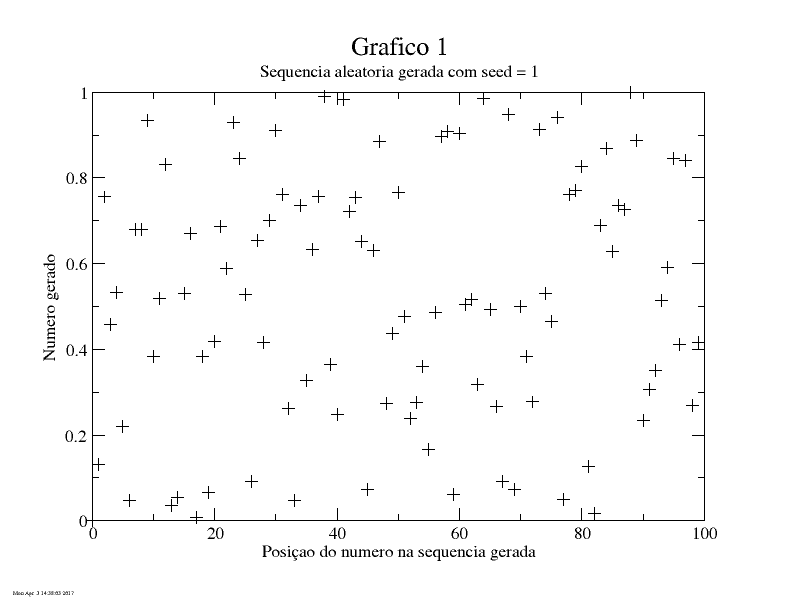
\includegraphics[width=\textwidth]{graf1}
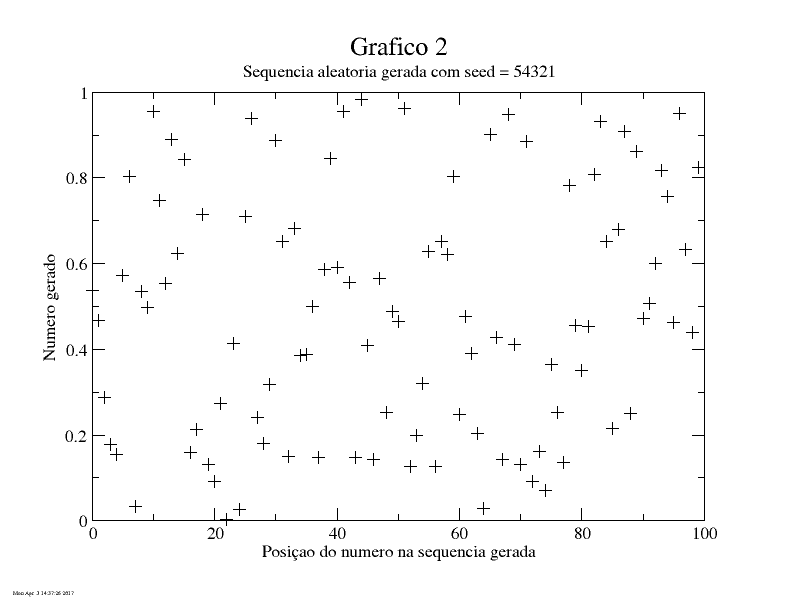
\includegraphics[width=\textwidth]{graf2}
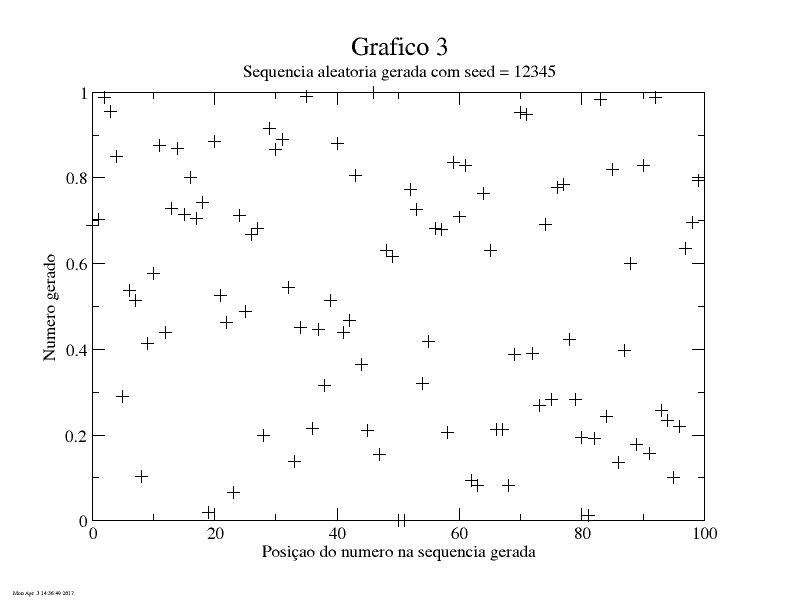
\includegraphics[width=\textwidth]{graf3}
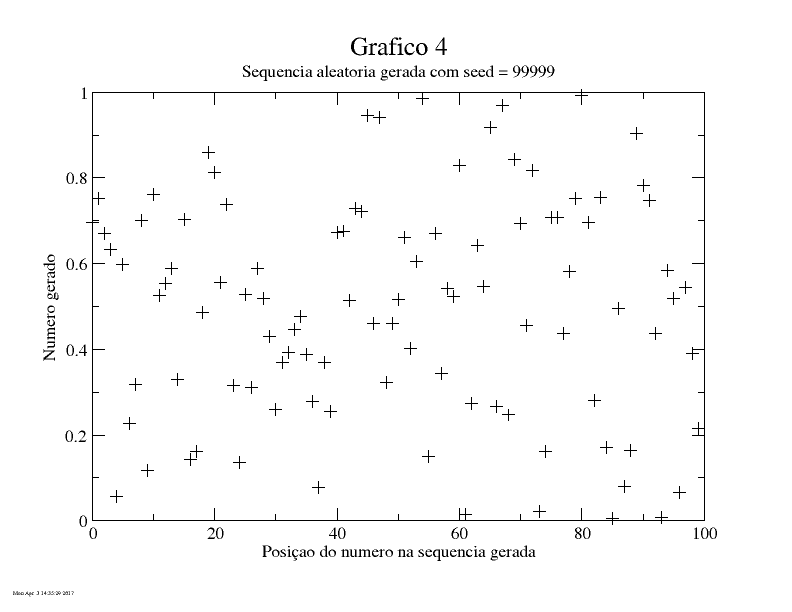
\includegraphics[width=\textwidth]{graf4}
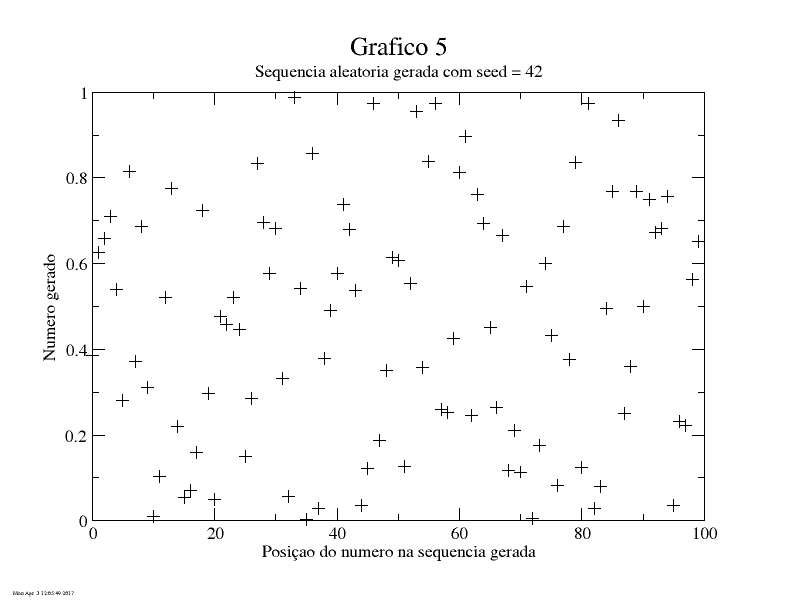
\includegraphics[width=\textwidth]{graf5}

Como esperado, a análise visual não revela nenhum padrão consistente nas representações gráficas. Tal desordem mostra-se útil em aplicações simples, menos formais, nas quais o rigor na aleatoriedade não se faz necessária.

\subsection{Decaimento radioativo}
O objetivo do vigente procedimento foi simular um processo de decaimento radioativo, por meio da produção de números pseudo-aleatórios.\par
Para esse programa, utilizou-se a função ran2, que gera números pseudo-aleatórios entre 0 e 1 com sementes diferentes a cada vez. Pode-se encontrá-la no site do Model, Analysis, and Prediction Program, da NASA (<\url{https://map.nasa.gov/GEOSgcm_f90toHTML/html_code/src/nr_ran2_gasdev.f90.html\}>, Acesso em: 6 abr 2017).\paragraph{}
A probabilidade $P$ de que um átomo decaia em um intervalo de tempo $dt$ se relaciona com o tempo de meia vida $\tau$ da seguinte forma:

\begin{equation}
  \label{eq:prob}
  dP=-\frac{1}{\tau}dt
\end{equation}

Definiu-se o tempo de meia vida como 1, de forma que a propabilidade de dcaimento euivale ao intervalo de tempo considerado, que, por sua vez, foi definido como 0.1. A quantidade inicial de átomos foi estabelecida como 1000, e o tempo máximo de simulação tmax, em quanto tempo esta chegará ao fim, será tomado como 8 (decidido a partir da observação dos resultados).\par
Elaborou-se laço que vai de t=1 até t=tmax/dt, e que gera R números aleatórios com a função ran2 e testa se foi obtido valor menor que $P$, incrementando em uma unidade uma variável de contagem caso a condicional se aplique. Tal processo corresponde à contar quantos àtomos decaíram em um intervalo de tempo.\par
Na fase seguinte, o número de átomos decaídos era subtraído da quantidade inicial de átomos, a variável de contagem era zerada, e o loop rodava novamente, para contar os que decairiam no intervalo de tempo seguinte. Observou-se que, na maioria das vezes, não restavam mais do que dois átomos em t=8, motivando a escolha tmax=8.\par
O procedimento foi repetido R = $10^4$ vezes (tratam-se, portanto, de dois laços DO encadeados), e foram calculadas a média ($\overline{x}$), desvio padrão:

\[\sigma =\sqrt{ \frac{1}{R} \sum_{i=1}^R (x_i - \overline{x})^2}\]

 e variância normalizada pela média, para cada intervalo de tempo. A variância normalizada é definida como o quadrado do desvio padrão sobre a média dos valores.\par
As 10 primeiras simulações e as médias de cada intervalo são compiladas no gráfico 6.

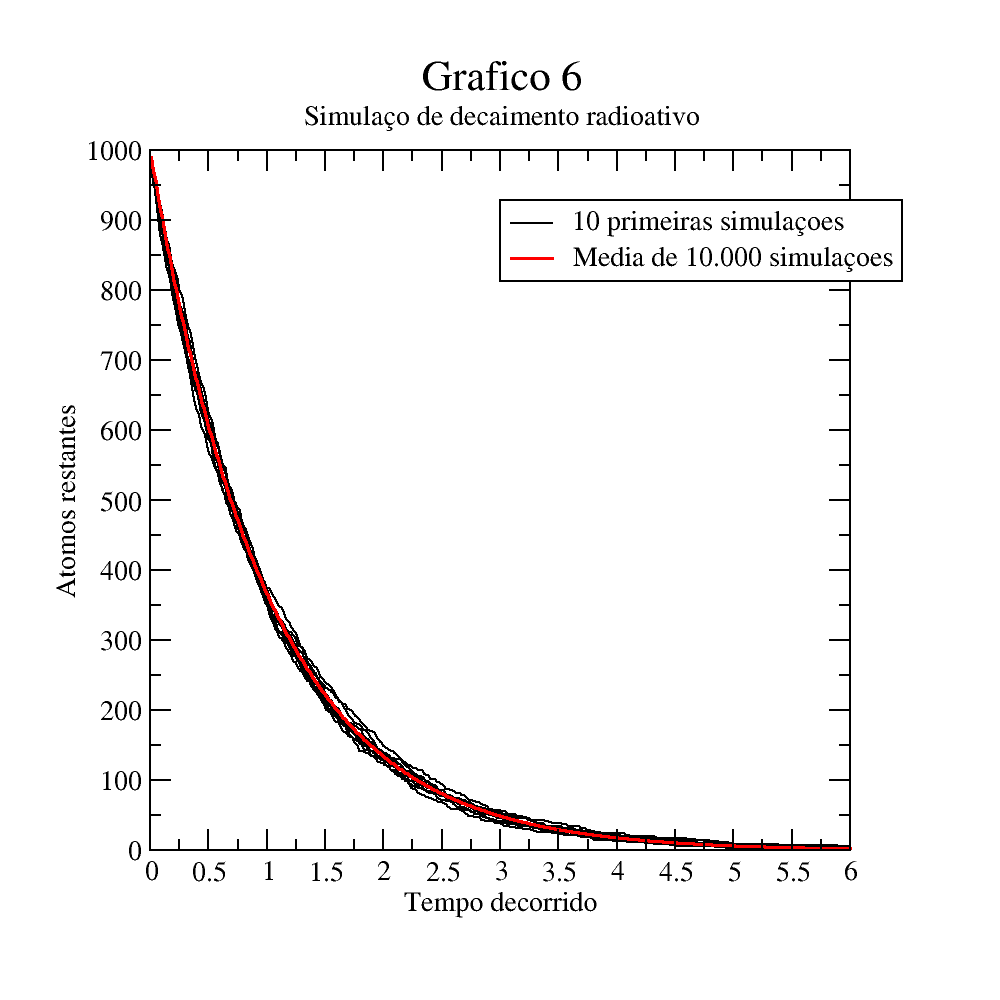
\includegraphics[width=\textwidth]{graf6}
A natureza exponencial do decaimento se torna clara pela visualização do gráfico 6, o que se explica pela relação mostrada pela equação \ref{eq:prob}.
Aproximando-se $dP$ para o número $dN$ de átomos decaídos no intervalo $dt$ sobre a quantidade total $N$ de átomos restantes e integrando-se a igualdade obtém-se:

\[dP=-\frac{1}{\tau}dt\]
\[\frac{dN}{N} =- \frac{1}{\tau}dt\]
\[\ln N = -\frac{t}{\tau} + t_0\]

Em que $t_0$ é o tempo inicial, que culmina, se definido como nulo, em 

\[N = e^{-\frac{t}{\tau}}\]
Resultado condizente com o comportamento do gráfico 6.

O desvio padrão e a variância normalizada para cada intervalo de tempo nos $10^4$ processos simulados são apresentados, respectivamente, pelos gráficos 7 e 8.

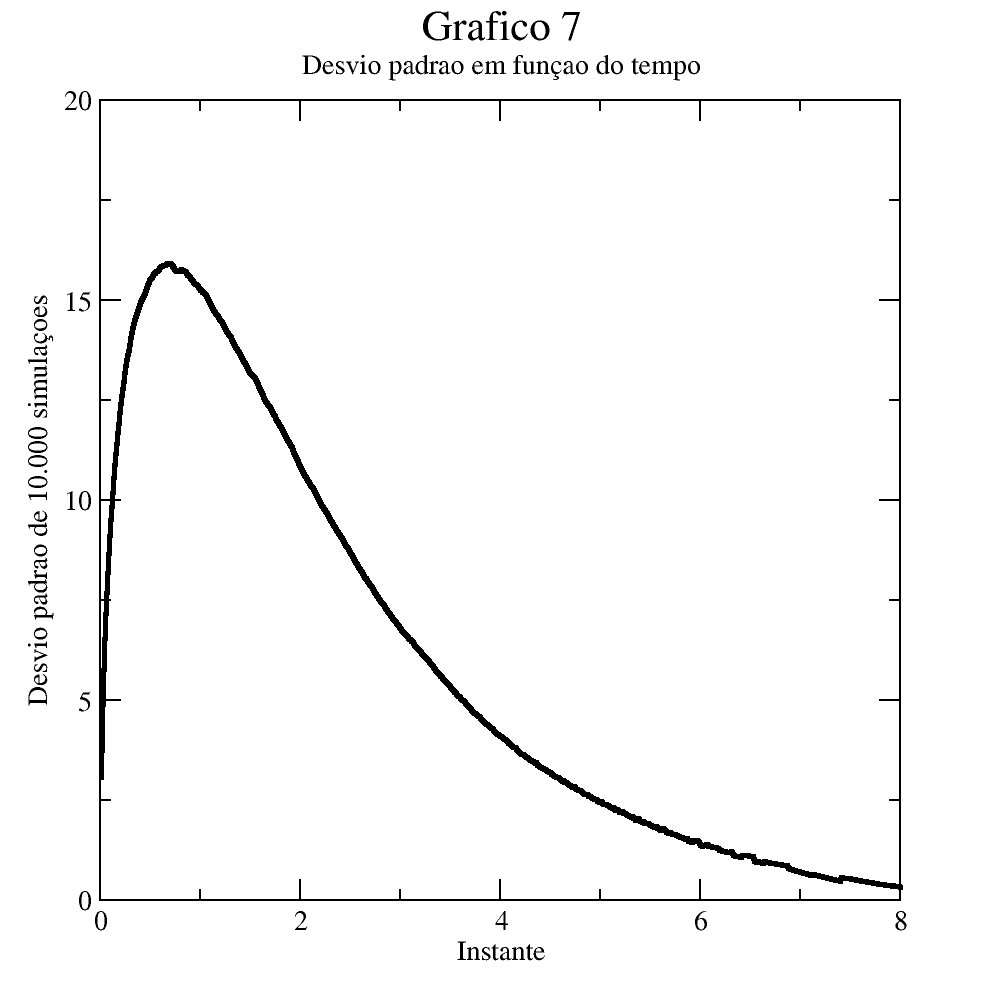
\includegraphics[width=\textwidth]{graf7}
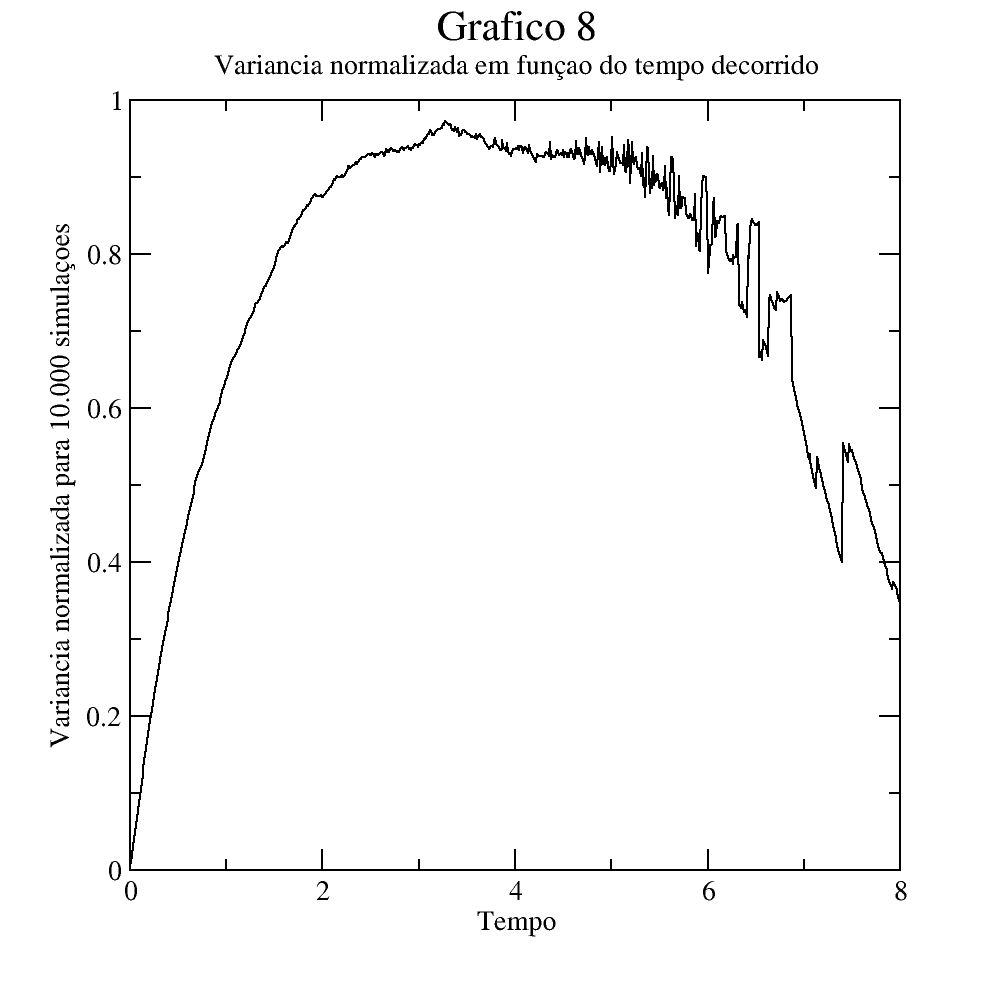
\includegraphics[width=\textwidth]{graf8}

Ambos tem valores iniciais nulos, visto que no primeiro instante, N era igual em todas as simulações. Em um primeiro momento, observa-se rápido crescimento nos dois gráficos visto que a quantidade de átomos decaídos em um intervalo depende da mesma quantidade no interalo anterior, e trantando-se de um processo aleatório, o desvio padrão dos valores tende a aumentar com o tempo.\par
Contudo como a quantidade de átomos decaídos tende a ser (dada as características estocásticas do conjunto) proporcional a N, ela tende a valores cada vez menores com o passar do tempo, já que N diminui. Isto é, a quantidade restante de átomos varia cada vez menos, levando o desvio padrão de N a convergir novamente, visto que o desvio padrão também depende de N.\par
A normalização com relação á média procura eliminar essa dependência de N na divergência dos valores, de forma que esperaríamos ver uma assíntota horizontal no gráfico 8.\par

Tanto o gráfico 7 como o 8 apresentam ruído, oscilações imprevisíveis dos valores, à medida que t aumenta. Isto se deve à perda de acuidade do desvio padrão conforme a razão entre a diferença entre os valores e os próprios valores aumenta ($\frac{dN}{N}$), ou seja, quando $dN$ torna-se significativa com relação a $N$, perde sua natureza diferencial. A normalização, originadora dos valores plotados em 8, amplifica esse fenômeno, fazendo com que o ruído ofusque completamente o caráter assintótico previsto para gráfico 8.\par

É possível relacional intuitivamente o espaçamento vertical entre as séries do gráfico 6 ao comportamento do desvio padrão mostrado no gráfico 7: ambos tem variação qualitativamente sincronizada.\par

Foi também elaborado o programa abaixo, que calcula uma matriz hist de dimensões 2 por R, que armazena, para um único intervalo de tempo, quantas vezes cada quantidade de átomos aparece entre as R amostras, sendo que a quantidade ocupa uma coluna e o numero de atomos a outra, e dados relacionados ocupam a mesma linha. Na grande maioria das vezes, não serão usadas todas as R linhas da matriz, e um condicional foi utilizado para imprimir somente os dados relevantes (descartar os itens nulos de hist).

\begin{lstlisting}

  !=========== HISTOGRAMA =============!
  
  allocate(hist(2,r))

do tesc= 100, 800, 100 ! loop mosntruoso

   !-------- limpa lixo ----------!
  do i=1, r
     hist(1,i) = 0
     hist(2,i) = 0
  end do
  !------------------------------!
  
  ! POS é a próxima posição que ainda não foi
  ! ocupada em hist, necessario para nao sobrescrever
  
  POS = 1

  inedito = .true.

  ! tesc é a posição do tempo escolhido
  ! (ex. se tesc = 5, teremos os dados
  ! referentes ao quinto instante:
  !       (5 * dt) = 0.5)

  do ri = 1, r
     do i =1, r
        if (mat(tesc, ri) .eq. hist(1,i)) then
           hist(2,i) = hist(2,i)+1
           inedito = .false.
           exit
        end if
     end do

     if (inedito) then
        hist(1, pos) = mat(tesc, ri)
        hist(2, pos) = 1
        pos = pos+1
     end if

     inedito=.true.
  end do
\end{lstlisting}

Fez-se necessário igualar todos os elementos da matriz a 0, inicialmente, pois o lixo de memória se constituiu um empecilho.
O programa foi rodado para diferentes intervalos, e os resultados são exibidos nos gráficos a seguir:

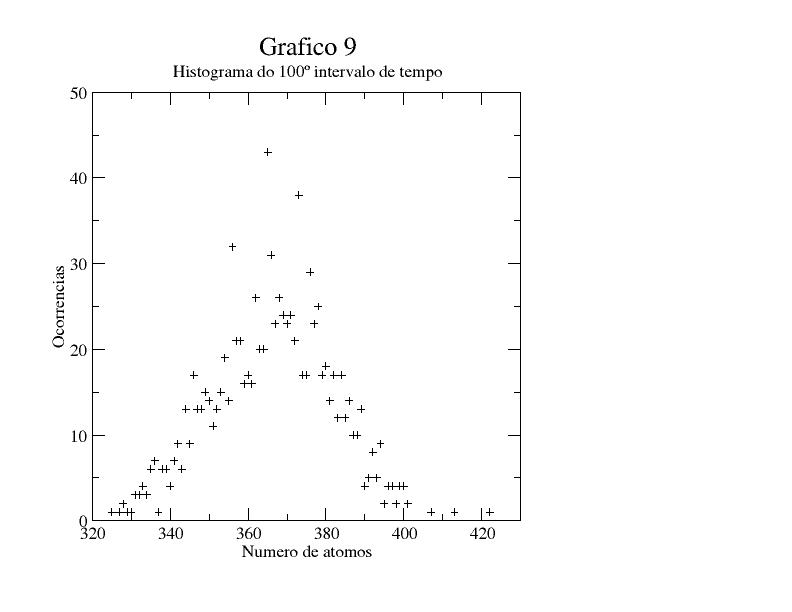
\includegraphics[width=\textwidth]{graf9}
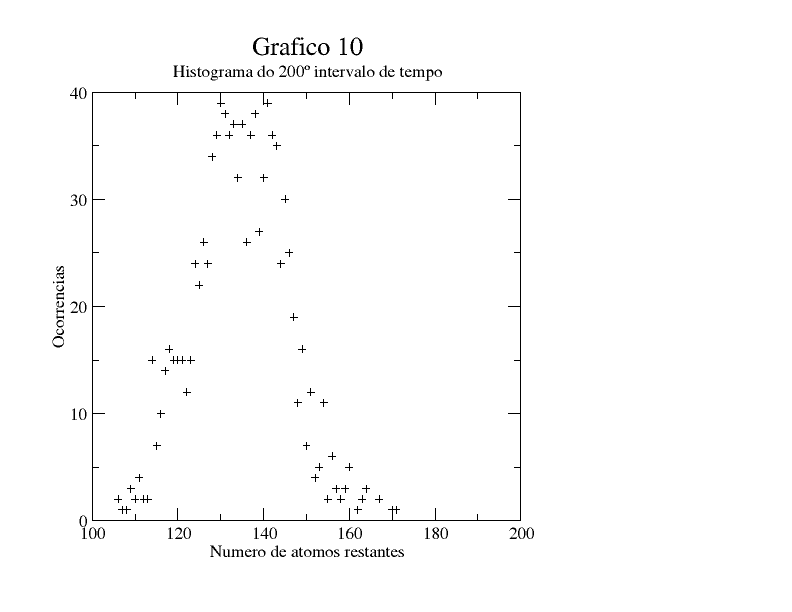
\includegraphics[width=\textwidth]{graf10}
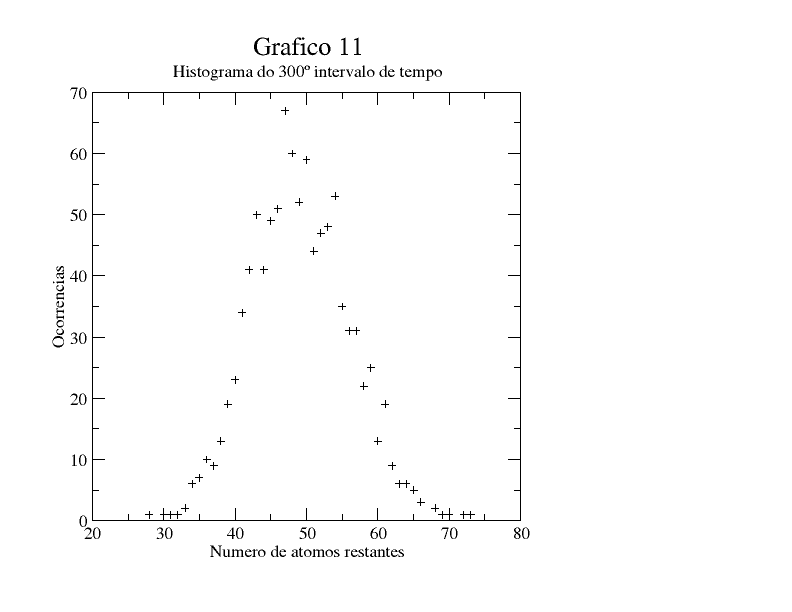
\includegraphics[width=\textwidth]{graf11}
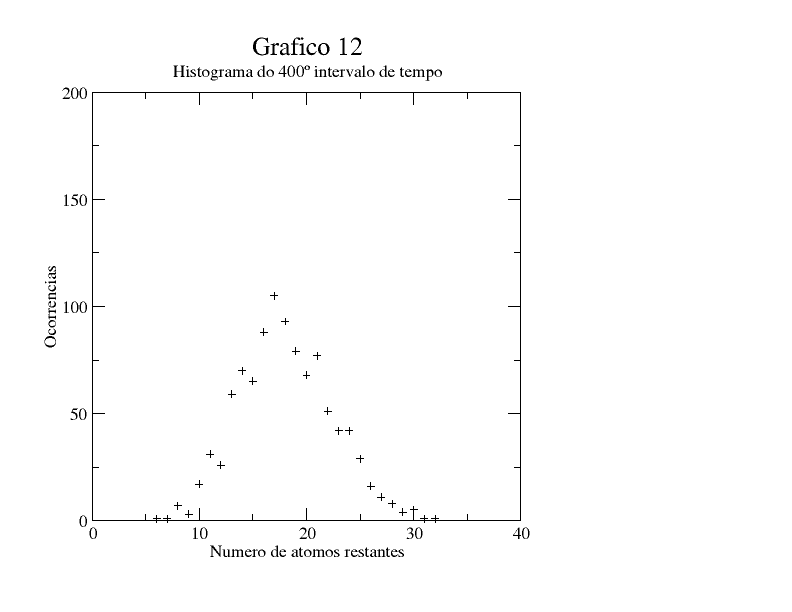
\includegraphics[width=\textwidth]{graf12}
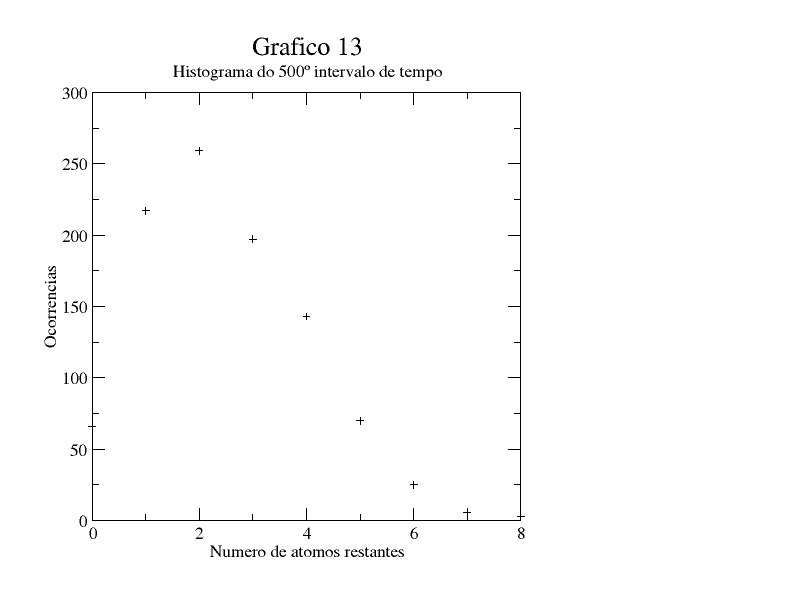
\includegraphics[width=\textwidth]{graf13}
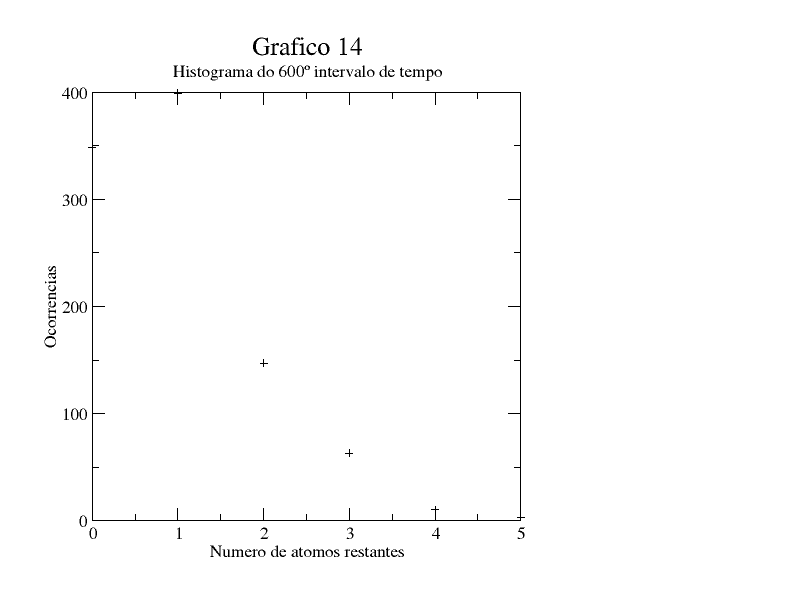
\includegraphics[width=\textwidth]{graf14}
\end{document}